\documentclass{beamer}

\usepackage[utf8]{inputenc}
\usepackage[english]{babel}
\usepackage[T1]{fontenc}
\usepackage{lmodern}
\usepackage{adjustbox}
\usepackage{graphicx}
\usepackage{commath}
\usepackage{amsmath,amssymb,amsthm}
\usepackage{tikz}
\usepackage{pgffor}
\usepackage[lined]{algorithm2e}
\usetheme{Singapore}
\newlength{\mylen}
\resetcounteronoverlays{compt}
\AtBeginSection[]
{
  \begin{frame}<beamer>
    \tableofcontents[currentsection]
  \end{frame}
}
\begin{document}

\title{Integrating lexical constraints and background knowledge to $K$-Means with Deep Learning}
\author{Maxence Grand \\                                                   
        Supervised by : \'Eric Gaussier  \and Marc Tommasi \and Aur\'elien Bellet \and Thibaut Thonet \and Maziar Moradi Fard} 
\institute{Laboratoire d'Informatique de Grenoble, Team AMA}
\date{\today}

\maketitle

\begin{frame}{Overview}
\tableofcontents
\end{frame}
\section{Introduction}

\begin{frame}
  \frametitle{Lexical Constraints}
  \pause
  \begin{itemize}
    \setlength\itemsep{2em}
  \item Set of keywords \pause
  \item Biais clustering
  \end{itemize}
\end{frame}
\begin{frame}
\frametitle{Background Knowledge}
\begin{itemize}
\pause
\item \textbf{Must-link} constraint $ML$ : $(X, X') \in ML \implies $ X and X' are in the
  same cluster.\pause
\item \textbf{Cannot-link} constraint $CL$ : $(X, X') \in CL \implies $ X and X' are in
  different cluster.
\end{itemize}
\end{frame}

\section{Related Work}

\begin{frame}
\frametitle{$K$-Means}
Given a corpus C, where each document X is a 
d-dimensional real vector, k-means clustering aims to partition the n 
documents into K $S_k$ clusters represented by centroids 
R = {$r_1, r_2, ..., r_K$}. :
Formally, the objective is to minimize :
$$
\sum_{k =1 }^K \sum_{X \in S_k} ||X - r_k||_2^2
$$
\end{frame}

\foreach \n in {0,...,11}{
  \begin{frame}
    \frametitle{$K$-Means}
  \begin{figure}[!h]
    \centering
    \includegraphics[scale=0.45]{kmeans/\n test.png}
  \end{figure}
  \end{frame}
}

\begin{frame}
  \frametitle{Auto-Encoder}
  \begin{columns}[T] % align columns
    \setlength{\mylen}{0.4\textwidth}
    \begin{column}{\mylen}
      \begin{figure}[!h]
        \centering
        \fbox{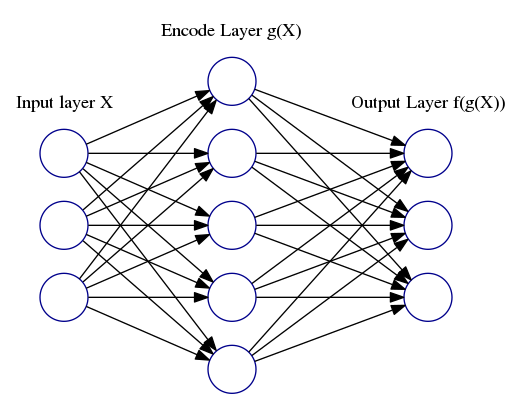
\includegraphics[scale=0.28]{autoencoder.png}}
        \caption{Auto-Encoder}
        \label{fig:AE}
      \end{figure}
    \end{column}%
    \hfill%
    \begin{column}{\dimexpr\textwidth-\mylen}
      \pause
      \begin{itemize}
        \setlength\itemsep{2em}
      \item Encode Function $g(X; \theta)$ \pause
      \item Decode Function $f(g(X; \theta)$ \pause
      \item $L_{rec}(X, \theta) = || X - f(g(X, \theta)) ||_2^2$
      \end{itemize}
    \end{column}%
  \end{columns}
\end{frame}

\begin{frame}
  \frametitle{Background Knowledge - COP$K$-Means}
  \begin{columns}[T] % align columns
    \setlength{\mylen}{0.5\textwidth}
    \begin{column}{\mylen}
      \scalebox{.7}{                        %new code
        \begin{algorithm}[H]
          \SetKwInOut{Input}{input}
          \SetKwInOut{Output}{output}
          \Input{Corpus C, must-link constraints $ML \subseteq C x C$,
            cannot-link constraints $CL \subseteq C x C$}
          \Output{Clusters $S_1, S_2, ..., S_k$}
          Let $S_1, S_2 , ..., S_k$ be the initial clusters\\
          \Repeat{Convergence}{
            \ForEach{$X_i \in C$}{
              Assign $X_i$ to closest $S_j$ such that Violate-Constraints($X_i, C_j, CL,
              ML$) is false.\\
              \If{No such clusters exists}{
                return \{\}\\
              }
            }
            \ForEach{Clusters $S_i$}{
              Update centroids.\\
            }
          }
          \Return{$S_1, S_2, ..., S_k$}
          \caption{\label{algo:cop}COP-Kmeans}
        \end{algorithm}  
      }
    \end{column}%
    \hfill%
    \begin{column}{\dimexpr\textwidth-\mylen}
      \scalebox{.7}{                        %new code
        \begin{algorithm}[H]
          \SetKwInOut{Input}{input}
          \SetKwInOut{Output}{output}
          \Input{Ducument X, Clusters S, must-link constraints $ML \subseteq C x C$,
            cannot-link constraints $CL \subseteq C x C$}
          \Output{True if constraints are violate, False otherwise}
          \ForEach{($X, X' \in ML$)}{
            \If{$X' \in S$}{
              \Return{True}
            }
          }
          \ForEach{($X, X' \in CL$)}{
            \If{$X' \in S$}{
              \Return{True}
            }
          }
          \Return{False}
          \caption{\label{algo:vio}Violate-Constraints}
        \end{algorithm}

      } 
    \end{column}%
  \end{columns}
\end{frame}

\begin{frame}
\frametitle{Background Knowledge - NNClustering}
\begin{figure}[!h]
  \centering
  \tikzset{every picture/.style={scale=0.8}}
  % Graphic for TeX using PGF
% Title: /media/maxence/SD_MAXENCE/cours/m1Informatique/S2/stage/soutenance/nnclust.dia
% Creator: Dia v0.97.3
% CreationDate: Fri Jun  8 11:45:14 2018
% For: maxence
% \usepackage{tikz}
% The following commands are not supported in PSTricks at present
% We define them conditionally, so when they are implemented,
% this pgf file will use them.
\ifx\du\undefined
  \newlength{\du}
\fi
\setlength{\du}{15\unitlength}
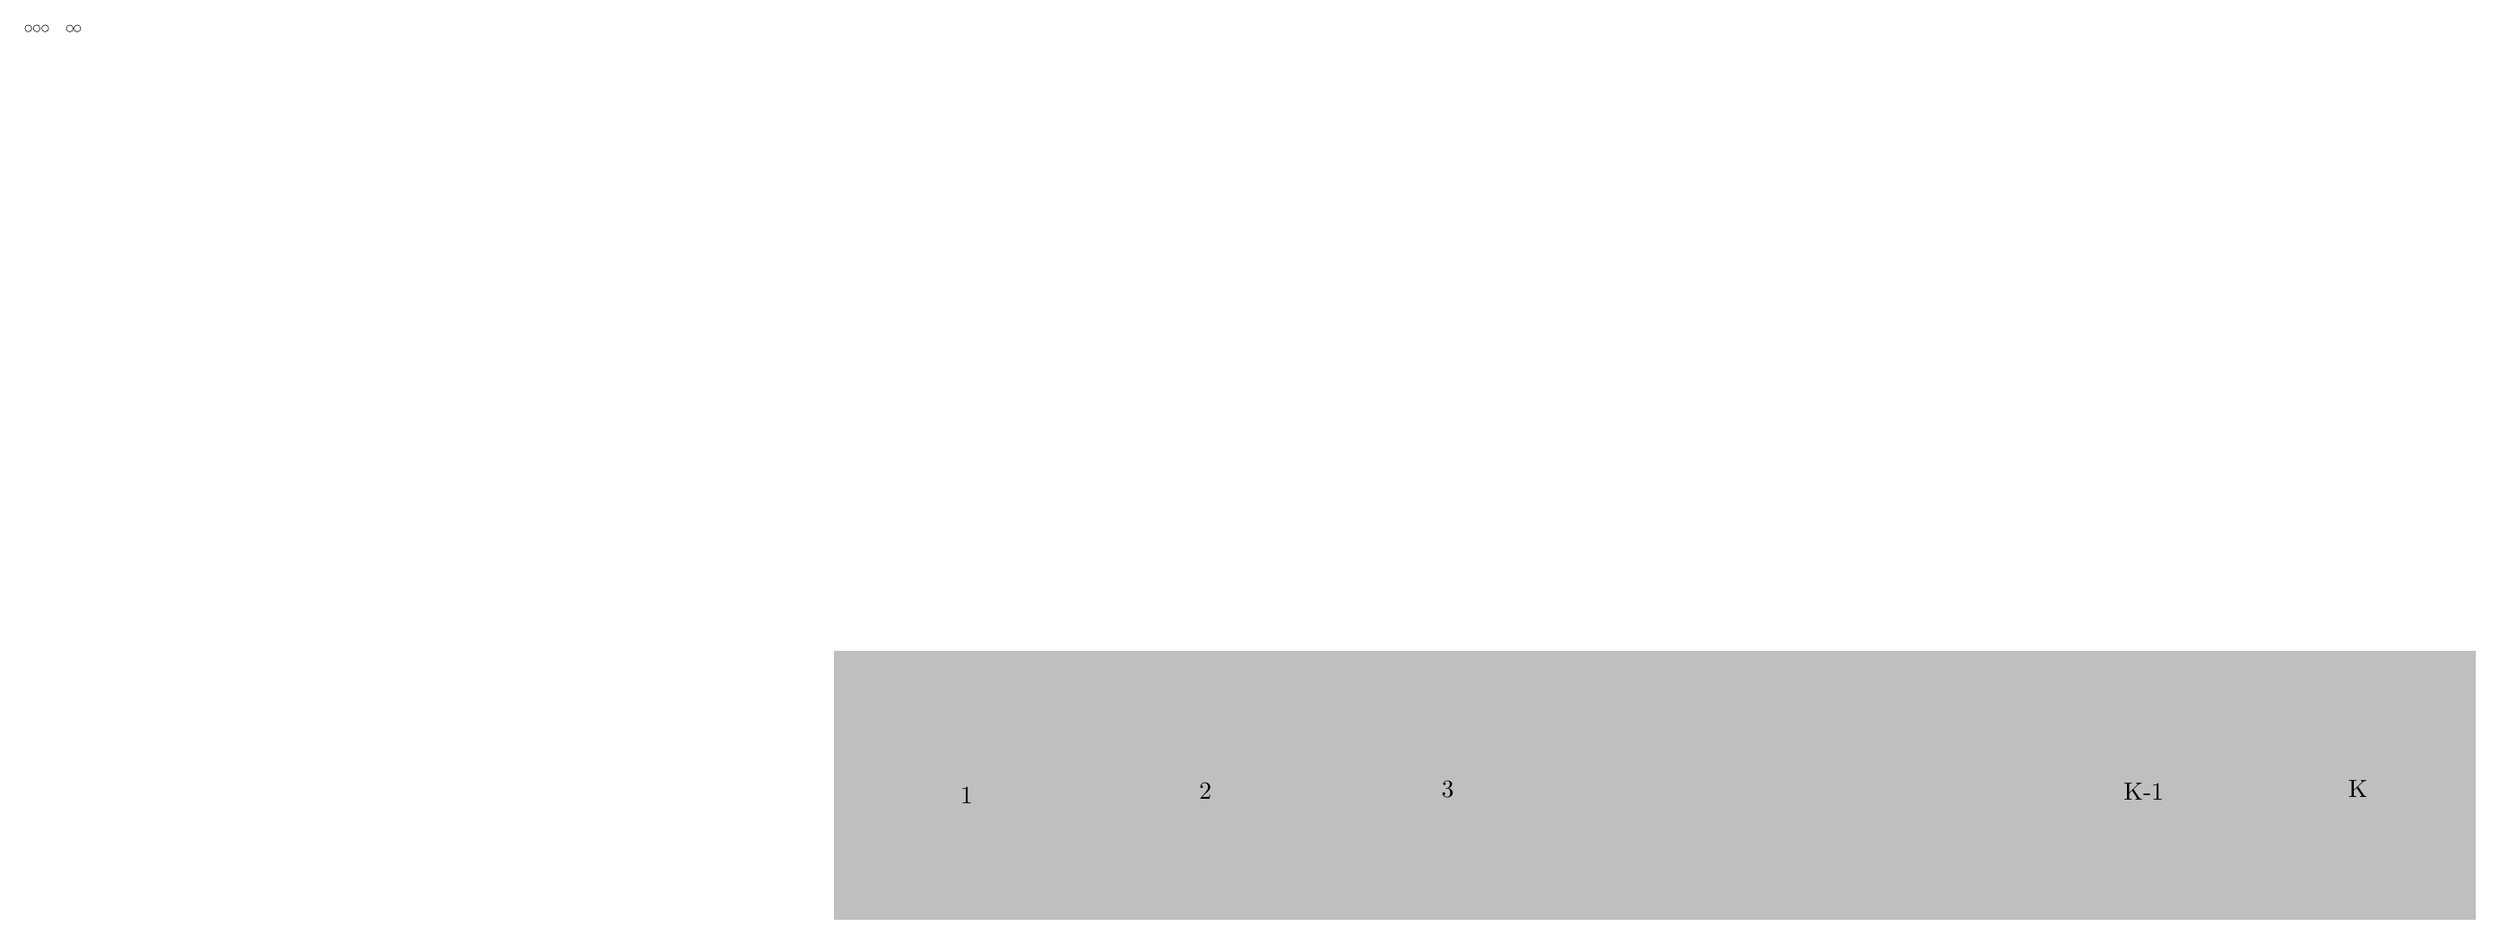
\begin{tikzpicture}
\pgftransformxscale{1.000000}
\pgftransformyscale{-1.000000}
\definecolor{dialinecolor}{rgb}{0.000000, 0.000000, 0.000000}
\pgfsetstrokecolor{dialinecolor}
\definecolor{dialinecolor}{rgb}{1.000000, 1.000000, 1.000000}
\pgfsetfillcolor{dialinecolor}
\definecolor{dialinecolor}{rgb}{0.749020, 0.749020, 0.749020}
\pgfsetfillcolor{dialinecolor}
\fill (11.900000\du,9.209061\du)--(11.900000\du,13.002312\du)--(35.134887\du,13.002312\du)--(35.134887\du,9.209061\du)--cycle;
\pgfsetlinewidth{0.100000\du}
\pgfsetdash{}{0pt}
\pgfsetdash{}{0pt}
\pgfsetmiterjoin
\definecolor{dialinecolor}{rgb}{0.749020, 0.749020, 0.749020}
\pgfsetstrokecolor{dialinecolor}
\draw (11.900000\du,9.209061\du)--(11.900000\du,13.002312\du)--(35.134887\du,13.002312\du)--(35.134887\du,9.209061\du)--cycle;
% setfont left to latex
\definecolor{dialinecolor}{rgb}{0.000000, 0.000000, 0.000000}
\pgfsetstrokecolor{dialinecolor}
\node at (23.517443\du,11.300687\du){};
\pgfsetlinewidth{0.100000\du}
\pgfsetdash{}{0pt}
\pgfsetdash{}{0pt}
\pgfsetbuttcap
\pgfsetmiterjoin
\pgfsetlinewidth{0.100000\du}
\pgfsetbuttcap
\pgfsetmiterjoin
\pgfsetdash{}{0pt}
\definecolor{dialinecolor}{rgb}{1.000000, 1.000000, 1.000000}
\pgfsetfillcolor{dialinecolor}
\pgfpathellipse{\pgfpoint{13.801924\du}{11.016529\du}}{\pgfpoint{1.385996\du}{0\du}}{\pgfpoint{0\du}{1.385996\du}}
\pgfusepath{fill}
\definecolor{dialinecolor}{rgb}{0.000000, 0.000000, 0.000000}
\pgfsetstrokecolor{dialinecolor}
\pgfpathellipse{\pgfpoint{13.801924\du}{11.016529\du}}{\pgfpoint{1.385996\du}{0\du}}{\pgfpoint{0\du}{1.385996\du}}
\pgfusepath{stroke}
\pgfsetbuttcap
\pgfsetmiterjoin
\pgfsetdash{}{0pt}
\definecolor{dialinecolor}{rgb}{0.000000, 0.000000, 0.000000}
\pgfsetstrokecolor{dialinecolor}
\pgfpathellipse{\pgfpoint{13.801924\du}{11.016529\du}}{\pgfpoint{1.385996\du}{0\du}}{\pgfpoint{0\du}{1.385996\du}}
\pgfusepath{stroke}
\pgfsetlinewidth{0.100000\du}
\pgfsetdash{}{0pt}
\pgfsetdash{}{0pt}
\pgfsetbuttcap
\pgfsetmiterjoin
\pgfsetlinewidth{0.100000\du}
\pgfsetbuttcap
\pgfsetmiterjoin
\pgfsetdash{}{0pt}
\definecolor{dialinecolor}{rgb}{1.000000, 1.000000, 1.000000}
\pgfsetfillcolor{dialinecolor}
\pgfpathellipse{\pgfpoint{17.168587\du}{10.998445\du}}{\pgfpoint{1.385996\du}{0\du}}{\pgfpoint{0\du}{1.385996\du}}
\pgfusepath{fill}
\definecolor{dialinecolor}{rgb}{0.000000, 0.000000, 0.000000}
\pgfsetstrokecolor{dialinecolor}
\pgfpathellipse{\pgfpoint{17.168587\du}{10.998445\du}}{\pgfpoint{1.385996\du}{0\du}}{\pgfpoint{0\du}{1.385996\du}}
\pgfusepath{stroke}
\pgfsetbuttcap
\pgfsetmiterjoin
\pgfsetdash{}{0pt}
\definecolor{dialinecolor}{rgb}{0.000000, 0.000000, 0.000000}
\pgfsetstrokecolor{dialinecolor}
\pgfpathellipse{\pgfpoint{17.168587\du}{10.998445\du}}{\pgfpoint{1.385996\du}{0\du}}{\pgfpoint{0\du}{1.385996\du}}
\pgfusepath{stroke}
\pgfsetlinewidth{0.100000\du}
\pgfsetdash{}{0pt}
\pgfsetdash{}{0pt}
\pgfsetbuttcap
\pgfsetmiterjoin
\pgfsetlinewidth{0.100000\du}
\pgfsetbuttcap
\pgfsetmiterjoin
\pgfsetdash{}{0pt}
\definecolor{dialinecolor}{rgb}{1.000000, 1.000000, 1.000000}
\pgfsetfillcolor{dialinecolor}
\pgfpathellipse{\pgfpoint{20.582513\du}{10.995203\du}}{\pgfpoint{1.385996\du}{0\du}}{\pgfpoint{0\du}{1.385996\du}}
\pgfusepath{fill}
\definecolor{dialinecolor}{rgb}{0.000000, 0.000000, 0.000000}
\pgfsetstrokecolor{dialinecolor}
\pgfpathellipse{\pgfpoint{20.582513\du}{10.995203\du}}{\pgfpoint{1.385996\du}{0\du}}{\pgfpoint{0\du}{1.385996\du}}
\pgfusepath{stroke}
\pgfsetbuttcap
\pgfsetmiterjoin
\pgfsetdash{}{0pt}
\definecolor{dialinecolor}{rgb}{0.000000, 0.000000, 0.000000}
\pgfsetstrokecolor{dialinecolor}
\pgfpathellipse{\pgfpoint{20.582513\du}{10.995203\du}}{\pgfpoint{1.385996\du}{0\du}}{\pgfpoint{0\du}{1.385996\du}}
\pgfusepath{stroke}
\pgfsetlinewidth{0.100000\du}
\pgfsetdash{}{0pt}
\pgfsetdash{}{0pt}
\pgfsetbuttcap
\pgfsetmiterjoin
\pgfsetlinewidth{0.100000\du}
\pgfsetbuttcap
\pgfsetmiterjoin
\pgfsetdash{}{0pt}
\definecolor{dialinecolor}{rgb}{1.000000, 1.000000, 1.000000}
\pgfsetfillcolor{dialinecolor}
\pgfpathellipse{\pgfpoint{30.467651\du}{11.030059\du}}{\pgfpoint{1.385996\du}{0\du}}{\pgfpoint{0\du}{1.385996\du}}
\pgfusepath{fill}
\definecolor{dialinecolor}{rgb}{0.000000, 0.000000, 0.000000}
\pgfsetstrokecolor{dialinecolor}
\pgfpathellipse{\pgfpoint{30.467651\du}{11.030059\du}}{\pgfpoint{1.385996\du}{0\du}}{\pgfpoint{0\du}{1.385996\du}}
\pgfusepath{stroke}
\pgfsetbuttcap
\pgfsetmiterjoin
\pgfsetdash{}{0pt}
\definecolor{dialinecolor}{rgb}{0.000000, 0.000000, 0.000000}
\pgfsetstrokecolor{dialinecolor}
\pgfpathellipse{\pgfpoint{30.467651\du}{11.030059\du}}{\pgfpoint{1.385996\du}{0\du}}{\pgfpoint{0\du}{1.385996\du}}
\pgfusepath{stroke}
\pgfsetlinewidth{0.100000\du}
\pgfsetdash{}{0pt}
\pgfsetdash{}{0pt}
\pgfsetbuttcap
\pgfsetmiterjoin
\pgfsetlinewidth{0.100000\du}
\pgfsetbuttcap
\pgfsetmiterjoin
\pgfsetdash{}{0pt}
\definecolor{dialinecolor}{rgb}{1.000000, 1.000000, 1.000000}
\pgfsetfillcolor{dialinecolor}
\pgfpathellipse{\pgfpoint{33.503866\du}{11.012227\du}}{\pgfpoint{1.385996\du}{0\du}}{\pgfpoint{0\du}{1.385996\du}}
\pgfusepath{fill}
\definecolor{dialinecolor}{rgb}{0.000000, 0.000000, 0.000000}
\pgfsetstrokecolor{dialinecolor}
\pgfpathellipse{\pgfpoint{33.503866\du}{11.012227\du}}{\pgfpoint{1.385996\du}{0\du}}{\pgfpoint{0\du}{1.385996\du}}
\pgfusepath{stroke}
\pgfsetbuttcap
\pgfsetmiterjoin
\pgfsetdash{}{0pt}
\definecolor{dialinecolor}{rgb}{0.000000, 0.000000, 0.000000}
\pgfsetstrokecolor{dialinecolor}
\pgfpathellipse{\pgfpoint{33.503866\du}{11.012227\du}}{\pgfpoint{1.385996\du}{0\du}}{\pgfpoint{0\du}{1.385996\du}}
\pgfusepath{stroke}
\pgfsetlinewidth{0.100000\du}
\pgfsetdash{}{0pt}
\pgfsetdash{}{0pt}
\pgfsetbuttcap
\pgfsetmiterjoin
\pgfsetlinewidth{0.100000\du}
\pgfsetbuttcap
\pgfsetmiterjoin
\pgfsetdash{}{0pt}
\definecolor{dialinecolor}{rgb}{1.000000, 1.000000, 1.000000}
\pgfsetfillcolor{dialinecolor}
\pgfpathmoveto{\pgfpoint{13.107057\du}{10.501587\du}}
\pgfpathlineto{\pgfpoint{14.440390\du}{10.501587\du}}
\pgfpathcurveto{\pgfpoint{14.624485\du}{10.501587\du}}{\pgfpoint{14.773724\du}{10.747831\du}}{\pgfpoint{14.773724\du}{11.051587\du}}
\pgfpathcurveto{\pgfpoint{14.773724\du}{11.355344\du}}{\pgfpoint{14.624485\du}{11.601587\du}}{\pgfpoint{14.440390\du}{11.601587\du}}
\pgfpathlineto{\pgfpoint{13.107057\du}{11.601587\du}}
\pgfpathcurveto{\pgfpoint{12.922962\du}{11.601587\du}}{\pgfpoint{12.773724\du}{11.355344\du}}{\pgfpoint{12.773724\du}{11.051587\du}}
\pgfpathcurveto{\pgfpoint{12.773724\du}{10.747831\du}}{\pgfpoint{12.922962\du}{10.501587\du}}{\pgfpoint{13.107057\du}{10.501587\du}}
\pgfusepath{fill}
\definecolor{dialinecolor}{rgb}{1.000000, 1.000000, 1.000000}
\pgfsetstrokecolor{dialinecolor}
\pgfpathmoveto{\pgfpoint{13.107057\du}{10.501587\du}}
\pgfpathlineto{\pgfpoint{14.440390\du}{10.501587\du}}
\pgfpathcurveto{\pgfpoint{14.624485\du}{10.501587\du}}{\pgfpoint{14.773724\du}{10.747831\du}}{\pgfpoint{14.773724\du}{11.051587\du}}
\pgfpathcurveto{\pgfpoint{14.773724\du}{11.355344\du}}{\pgfpoint{14.624485\du}{11.601587\du}}{\pgfpoint{14.440390\du}{11.601587\du}}
\pgfpathlineto{\pgfpoint{13.107057\du}{11.601587\du}}
\pgfpathcurveto{\pgfpoint{12.922962\du}{11.601587\du}}{\pgfpoint{12.773724\du}{11.355344\du}}{\pgfpoint{12.773724\du}{11.051587\du}}
\pgfpathcurveto{\pgfpoint{12.773724\du}{10.747831\du}}{\pgfpoint{12.922962\du}{10.501587\du}}{\pgfpoint{13.107057\du}{10.501587\du}}
\pgfusepath{stroke}
% setfont left to latex
\definecolor{dialinecolor}{rgb}{0.000000, 0.000000, 0.000000}
\pgfsetstrokecolor{dialinecolor}
\node at (13.773724\du,11.251587\du){1};
\pgfsetlinewidth{0.100000\du}
\pgfsetdash{}{0pt}
\pgfsetdash{}{0pt}
\pgfsetbuttcap
\pgfsetmiterjoin
\pgfsetlinewidth{0.100000\du}
\pgfsetbuttcap
\pgfsetmiterjoin
\pgfsetdash{}{0pt}
\definecolor{dialinecolor}{rgb}{1.000000, 1.000000, 1.000000}
\pgfsetfillcolor{dialinecolor}
\pgfpathmoveto{\pgfpoint{16.489547\du}{10.449088\du}}
\pgfpathlineto{\pgfpoint{17.822881\du}{10.449088\du}}
\pgfpathcurveto{\pgfpoint{18.006976\du}{10.449088\du}}{\pgfpoint{18.156214\du}{10.695331\du}}{\pgfpoint{18.156214\du}{10.999088\du}}
\pgfpathcurveto{\pgfpoint{18.156214\du}{11.302845\du}}{\pgfpoint{18.006976\du}{11.549088\du}}{\pgfpoint{17.822881\du}{11.549088\du}}
\pgfpathlineto{\pgfpoint{16.489547\du}{11.549088\du}}
\pgfpathcurveto{\pgfpoint{16.305452\du}{11.549088\du}}{\pgfpoint{16.156214\du}{11.302845\du}}{\pgfpoint{16.156214\du}{10.999088\du}}
\pgfpathcurveto{\pgfpoint{16.156214\du}{10.695331\du}}{\pgfpoint{16.305452\du}{10.449088\du}}{\pgfpoint{16.489547\du}{10.449088\du}}
\pgfusepath{fill}
\definecolor{dialinecolor}{rgb}{1.000000, 1.000000, 1.000000}
\pgfsetstrokecolor{dialinecolor}
\pgfpathmoveto{\pgfpoint{16.489547\du}{10.449088\du}}
\pgfpathlineto{\pgfpoint{17.822881\du}{10.449088\du}}
\pgfpathcurveto{\pgfpoint{18.006976\du}{10.449088\du}}{\pgfpoint{18.156214\du}{10.695331\du}}{\pgfpoint{18.156214\du}{10.999088\du}}
\pgfpathcurveto{\pgfpoint{18.156214\du}{11.302845\du}}{\pgfpoint{18.006976\du}{11.549088\du}}{\pgfpoint{17.822881\du}{11.549088\du}}
\pgfpathlineto{\pgfpoint{16.489547\du}{11.549088\du}}
\pgfpathcurveto{\pgfpoint{16.305452\du}{11.549088\du}}{\pgfpoint{16.156214\du}{11.302845\du}}{\pgfpoint{16.156214\du}{10.999088\du}}
\pgfpathcurveto{\pgfpoint{16.156214\du}{10.695331\du}}{\pgfpoint{16.305452\du}{10.449088\du}}{\pgfpoint{16.489547\du}{10.449088\du}}
\pgfusepath{stroke}
% setfont left to latex
\definecolor{dialinecolor}{rgb}{0.000000, 0.000000, 0.000000}
\pgfsetstrokecolor{dialinecolor}
\node at (17.156214\du,11.199088\du){2};
\pgfsetlinewidth{0.100000\du}
\pgfsetdash{}{0pt}
\pgfsetdash{}{0pt}
\pgfsetbuttcap
\pgfsetmiterjoin
\pgfsetlinewidth{0.100000\du}
\pgfsetbuttcap
\pgfsetmiterjoin
\pgfsetdash{}{0pt}
\definecolor{dialinecolor}{rgb}{1.000000, 1.000000, 1.000000}
\pgfsetfillcolor{dialinecolor}
\pgfpathmoveto{\pgfpoint{19.922037\du}{10.421588\du}}
\pgfpathlineto{\pgfpoint{21.255370\du}{10.421588\du}}
\pgfpathcurveto{\pgfpoint{21.439465\du}{10.421588\du}}{\pgfpoint{21.588704\du}{10.667831\du}}{\pgfpoint{21.588704\du}{10.971588\du}}
\pgfpathcurveto{\pgfpoint{21.588704\du}{11.275345\du}}{\pgfpoint{21.439465\du}{11.521588\du}}{\pgfpoint{21.255370\du}{11.521588\du}}
\pgfpathlineto{\pgfpoint{19.922037\du}{11.521588\du}}
\pgfpathcurveto{\pgfpoint{19.737942\du}{11.521588\du}}{\pgfpoint{19.588704\du}{11.275345\du}}{\pgfpoint{19.588704\du}{10.971588\du}}
\pgfpathcurveto{\pgfpoint{19.588704\du}{10.667831\du}}{\pgfpoint{19.737942\du}{10.421588\du}}{\pgfpoint{19.922037\du}{10.421588\du}}
\pgfusepath{fill}
\definecolor{dialinecolor}{rgb}{1.000000, 1.000000, 1.000000}
\pgfsetstrokecolor{dialinecolor}
\pgfpathmoveto{\pgfpoint{19.922037\du}{10.421588\du}}
\pgfpathlineto{\pgfpoint{21.255370\du}{10.421588\du}}
\pgfpathcurveto{\pgfpoint{21.439465\du}{10.421588\du}}{\pgfpoint{21.588704\du}{10.667831\du}}{\pgfpoint{21.588704\du}{10.971588\du}}
\pgfpathcurveto{\pgfpoint{21.588704\du}{11.275345\du}}{\pgfpoint{21.439465\du}{11.521588\du}}{\pgfpoint{21.255370\du}{11.521588\du}}
\pgfpathlineto{\pgfpoint{19.922037\du}{11.521588\du}}
\pgfpathcurveto{\pgfpoint{19.737942\du}{11.521588\du}}{\pgfpoint{19.588704\du}{11.275345\du}}{\pgfpoint{19.588704\du}{10.971588\du}}
\pgfpathcurveto{\pgfpoint{19.588704\du}{10.667831\du}}{\pgfpoint{19.737942\du}{10.421588\du}}{\pgfpoint{19.922037\du}{10.421588\du}}
\pgfusepath{stroke}
% setfont left to latex
\definecolor{dialinecolor}{rgb}{0.000000, 0.000000, 0.000000}
\pgfsetstrokecolor{dialinecolor}
\node at (20.588704\du,11.171588\du){3};
\pgfsetlinewidth{0.100000\du}
\pgfsetdash{}{0pt}
\pgfsetdash{}{0pt}
\pgfsetbuttcap
\pgfsetmiterjoin
\pgfsetlinewidth{0.100000\du}
\pgfsetbuttcap
\pgfsetmiterjoin
\pgfsetdash{}{0pt}
\definecolor{dialinecolor}{rgb}{1.000000, 1.000000, 1.000000}
\pgfsetfillcolor{dialinecolor}
\pgfpathmoveto{\pgfpoint{29.779508\du}{10.444088\du}}
\pgfpathlineto{\pgfpoint{31.112841\du}{10.444088\du}}
\pgfpathcurveto{\pgfpoint{31.296936\du}{10.444088\du}}{\pgfpoint{31.446175\du}{10.690331\du}}{\pgfpoint{31.446175\du}{10.994088\du}}
\pgfpathcurveto{\pgfpoint{31.446175\du}{11.297845\du}}{\pgfpoint{31.296936\du}{11.544088\du}}{\pgfpoint{31.112841\du}{11.544088\du}}
\pgfpathlineto{\pgfpoint{29.779508\du}{11.544088\du}}
\pgfpathcurveto{\pgfpoint{29.595413\du}{11.544088\du}}{\pgfpoint{29.446175\du}{11.297845\du}}{\pgfpoint{29.446175\du}{10.994088\du}}
\pgfpathcurveto{\pgfpoint{29.446175\du}{10.690331\du}}{\pgfpoint{29.595413\du}{10.444088\du}}{\pgfpoint{29.779508\du}{10.444088\du}}
\pgfusepath{fill}
\definecolor{dialinecolor}{rgb}{1.000000, 1.000000, 1.000000}
\pgfsetstrokecolor{dialinecolor}
\pgfpathmoveto{\pgfpoint{29.779508\du}{10.444088\du}}
\pgfpathlineto{\pgfpoint{31.112841\du}{10.444088\du}}
\pgfpathcurveto{\pgfpoint{31.296936\du}{10.444088\du}}{\pgfpoint{31.446175\du}{10.690331\du}}{\pgfpoint{31.446175\du}{10.994088\du}}
\pgfpathcurveto{\pgfpoint{31.446175\du}{11.297845\du}}{\pgfpoint{31.296936\du}{11.544088\du}}{\pgfpoint{31.112841\du}{11.544088\du}}
\pgfpathlineto{\pgfpoint{29.779508\du}{11.544088\du}}
\pgfpathcurveto{\pgfpoint{29.595413\du}{11.544088\du}}{\pgfpoint{29.446175\du}{11.297845\du}}{\pgfpoint{29.446175\du}{10.994088\du}}
\pgfpathcurveto{\pgfpoint{29.446175\du}{10.690331\du}}{\pgfpoint{29.595413\du}{10.444088\du}}{\pgfpoint{29.779508\du}{10.444088\du}}
\pgfusepath{stroke}
% setfont left to latex
\definecolor{dialinecolor}{rgb}{0.000000, 0.000000, 0.000000}
\pgfsetstrokecolor{dialinecolor}
\node at (30.446175\du,11.194088\du){K-1};
\pgfsetlinewidth{0.100000\du}
\pgfsetdash{}{0pt}
\pgfsetdash{}{0pt}
\pgfsetbuttcap
\pgfsetmiterjoin
\pgfsetlinewidth{0.100000\du}
\pgfsetbuttcap
\pgfsetmiterjoin
\pgfsetdash{}{0pt}
\definecolor{dialinecolor}{rgb}{1.000000, 1.000000, 1.000000}
\pgfsetfillcolor{dialinecolor}
\pgfpathmoveto{\pgfpoint{32.811999\du}{10.416588\du}}
\pgfpathlineto{\pgfpoint{34.145332\du}{10.416588\du}}
\pgfpathcurveto{\pgfpoint{34.329427\du}{10.416588\du}}{\pgfpoint{34.478666\du}{10.662831\du}}{\pgfpoint{34.478666\du}{10.966588\du}}
\pgfpathcurveto{\pgfpoint{34.478666\du}{11.270345\du}}{\pgfpoint{34.329427\du}{11.516588\du}}{\pgfpoint{34.145332\du}{11.516588\du}}
\pgfpathlineto{\pgfpoint{32.811999\du}{11.516588\du}}
\pgfpathcurveto{\pgfpoint{32.627904\du}{11.516588\du}}{\pgfpoint{32.478666\du}{11.270345\du}}{\pgfpoint{32.478666\du}{10.966588\du}}
\pgfpathcurveto{\pgfpoint{32.478666\du}{10.662831\du}}{\pgfpoint{32.627904\du}{10.416588\du}}{\pgfpoint{32.811999\du}{10.416588\du}}
\pgfusepath{fill}
\definecolor{dialinecolor}{rgb}{1.000000, 1.000000, 1.000000}
\pgfsetstrokecolor{dialinecolor}
\pgfpathmoveto{\pgfpoint{32.811999\du}{10.416588\du}}
\pgfpathlineto{\pgfpoint{34.145332\du}{10.416588\du}}
\pgfpathcurveto{\pgfpoint{34.329427\du}{10.416588\du}}{\pgfpoint{34.478666\du}{10.662831\du}}{\pgfpoint{34.478666\du}{10.966588\du}}
\pgfpathcurveto{\pgfpoint{34.478666\du}{11.270345\du}}{\pgfpoint{34.329427\du}{11.516588\du}}{\pgfpoint{34.145332\du}{11.516588\du}}
\pgfpathlineto{\pgfpoint{32.811999\du}{11.516588\du}}
\pgfpathcurveto{\pgfpoint{32.627904\du}{11.516588\du}}{\pgfpoint{32.478666\du}{11.270345\du}}{\pgfpoint{32.478666\du}{10.966588\du}}
\pgfpathcurveto{\pgfpoint{32.478666\du}{10.662831\du}}{\pgfpoint{32.627904\du}{10.416588\du}}{\pgfpoint{32.811999\du}{10.416588\du}}
\pgfusepath{stroke}
% setfont left to latex
\definecolor{dialinecolor}{rgb}{0.000000, 0.000000, 0.000000}
\pgfsetstrokecolor{dialinecolor}
\node at (33.478666\du,11.166588\du){K};
\end{tikzpicture}

  \label{fig:archi}
\end{figure}
\end{frame}
\begin{frame}
\frametitle{Background Knowledge - NNClustering}
\begin{equation*}
  P = f(x_p), ~ Q = f(x_q)
\end{equation*}
\pause
\begin{equation*}
  KL(P||Q) = \sum_i^k P_ilog\frac{P_i}{Q_i}
\end{equation*}
\pause
\begin{equation*}
  I_s = \left\{
\begin{array}{ll}
  1 & \mbox{if $x_p$ and $x_q$ is a similar pair}\\
  0 & \mbox{Otherwise.}
\end{array}
\right.
\end{equation*}
%
\begin{equation*}
  I_{ds} = \left\{
\begin{array}{ll}
  1 & \mbox{if $x_p$ and $x_q$ is a dissimilar pair}\\
  0 & \mbox{Otherwise.}
\end{array}
\right.
\end{equation*}
\begin{equation*}
  Loss(P || Q) = I_s(x_p, x_q)KL(P || Q) + I_{ds}(x_p, x_q)max(0,
  \eta-KL(P||Q))
\end{equation*}
\begin{equation*}
  L(P,Q) = Loss(P || Q) + Loss(Q || P)
\end{equation*}
\end{frame}


\begin{frame}
\frametitle{Deep Clustering - General Form}
\begin{itemize}
\item \textbf{Non-Clustering loss} : $L_{NonClust}(C;\theta)$
\item \textbf{Clustering loss} : $L_{Clust}(C;\theta)$
\end{itemize}
\pause
The loss function takes the form :
\begin{equation*}
L(X;\theta) = \lambda L_{NonClust}(C;\theta) + (1-\lambda)L_{Clust}(C; \theta)
\end{equation*}
Where $\lambda \in [0 ; 1]$

\end{frame}
\begin{frame}
  \frametitle{Deep $K$-Means }
\begin{equation*}
L(C ,\beta;\theta,R) = L_{NonClust}(C;\theta,R ) + \lambda L_{Clust}(C,\beta;\theta,R)
\end{equation*}
\begin{equation*}
L_{NonClust}(C;\theta,R ) = \sum_{X \in C} ||X - f(g(X;\theta))||_2^2
\end{equation*}
\begin{equation*}
  L_{Clust}(C,\beta;\theta,R) = \sum_{X \in C} F(g(X),c(g(X, \theta); R))
\end{equation*}
\end{frame}

\begin{frame}
  \frametitle{Deep $K$-Means }
\begin{equation*}
L_{Clust} = \sum_{X \in C} \sum_{k=1}^K F(g(X; \theta), r_k) G_{k, F}(g(X; \theta), \beta; R)
\end{equation*}
\begin{equation*}
G_{k, F}(g(X; \theta), \beta; R) = \frac{e^{-\beta F(g(X, \theta),r_k)}}
{\sum_{k' = 1}^K e^{-\beta F(g(X, \theta),r_k')}}
\end{equation*}
\end{frame}
\section{Proposed Method}

\begin{frame}
\frametitle{The Idea}
Learn a latent space taking into account lexical constraints and
background knowledge.
\pause
\begin{equation*}\label{eq:h}
  h_X = g(X,\theta)
\end{equation*}
\end{frame}

\begin{frame}
\frametitle{Lexical Constraints}
\begin{equation*}
KW = \begin{pmatrix} kw_1 & kw_2 & ... & kw_{N_{kw}-1} & kw_{N_{kw}}
\end {pmatrix}
\end{equation*}
\pause
Introducing $X'$ such that
\begin{equation*}
\forall_{i=1,2,..,n}X_i' = \left\{
\begin{array}{ll}
  X_i & \mbox{if } i \in KW \\
  0 & \mbox{Otherwise.}
\end{array}
\right.
\end{equation*}
\pause
\begin{equation*}\label{eq:omega1}
  \omega_{KW} = \sum_{X \in C} || h_{X} - h_{X'}||_2^2
\end{equation*}
\end{frame}

\begin{frame}
\frametitle{Background Knowledge}
\pause
\begin{itemize}
\item Must-Link : $$\omega_{ML} = \sum_{\forall{(X_i,X_j)\in ML}} || h_{X_i} - h_{X_j} ||_2^2$$ \pause
\item Cannot-Link : $$\omega_{CL} = \sum_{\forall{(X_i,X_j)\in CL}} max(0,
  \eta - || h_{X_i} - h_{X_j} ||_2^2)$$
\end{itemize}
\end{frame}

\begin{frame}
\frametitle{Non Clustering Loss}
\begin{equation*}\label{eq:Sparse}
  \Omega(C, KW;\theta) = \alpha_0\omega_{KW} + \alpha_1\omega_{CL} + \alpha_2\omega_{ML}  
\end{equation*}
\pause
\begin{equation*}
  L_{rec}(C, \theta) = \sum_{X \in C}(||X - f(g(X, \theta))||_2^2
\end{equation*}
\pause
\begin{equation*}
  L_{NonClust}(C,KW; \theta) = L_{rec}(C, \theta) + \Omega(C)  
\end{equation*}

\end{frame}

\begin{frame}
\frametitle{Deep $K$-Means}
$$R = \begin{pmatrix} r_1 & r_2 & ... & r_K\end{pmatrix}$$
\pause
\begin{equation*}
  L_{Clust}(C, K, \beta; \theta, R) = \sum_{X \in C}\sum_{k=1}^K F(h_X, r_k) G_{k, F}(h_X, \beta; R) 
\end{equation*}
\pause
\begin{equation*}
  Min~L(KW, C, K; \theta) = L_{NonClust}(C, KW; \theta) + \lambda.L_{clust}(C, K, \beta; \theta, R)
\end{equation*}
with $\lambda \geq 0$
\end{frame}

\section{Experiment}

\begin{frame}
  \frametitle{Data}
  \begin{itemize}
    \setlength\itemsep{2em}
  \item 20 newsgroup
  \item RCV1 
  \end{itemize}
\end{frame}

\begin{frame}
\frametitle{Generate Lexical Constraints}
\scalebox{.7}{
\begin{algorithm}[H]
  \SetKwInOut{Input}{input}
  \SetKwInOut{Output}{output}
  \Input{Corpus C, The number of keywords per classes $P$}
  \Output{KW}
  $KW \gets \{\}$\\
  \ForEach{Class $c_i \in C$}{
    $rank_i \gets [0 ... 0]$\\
    \ForEach{Document $X \in c_i$}{
      \ForEach{Word $w \in X$}{
        $rank_{i,w} \gets rank_{i,w} + TFIDF(w,X, C)$\\
      }
    }
  }
  \ForEach{Class $c_i, c_j \in C$}{
    \If{$c_i \neq c_j$}{
      $rank_i \gets rank_i - rank_j$\\
    }
  }
  \ForEach{Class $c_i \in C$}{
    $KW \gets KW \cup \{\{w_1, w_2 ... w_P\} : \not\exists (v_1, v_2) | v_1 \not\in 
    \{w_1, w_2 ... w_P\}, v_2 \in \{w_1, w_2 ... w_P\}, rank_{i,v_1} \ge rank_{i,v_2}\}$\\
  }
  \Return{KW}
  \caption{\label{algo:gen_kw}Extract Keywords}
\end{algorithm}
}
\end{frame}

\begin{frame}
\frametitle{Metric}
\pause
\begin{itemize}
\item NMI :
$$NMI(S,C) = \frac{I(S,C)}{[H(S)+H(C)]/2}$$ 
with
$I(S,C) =\sum_k \sum_f\frac{|s_k \cap c_f|}{N}log\frac{N|s_k \cap c_f|}{|s_k| |c_f|}$
and
$H(S) = -\sum_k\frac{|s_k|}{N}log\frac{N|s_k|}{|s_k|}$
\pause
\item Accuracy :
$$
ACC(S,C) = \frac{1}{N}\sum_k {max}_j|s_k \cap c_j|
$$
\pause
\item Adjusted Rand Index :
$$ARI = \frac{a+b}{\binom{N}{2}}$$
\end{itemize}
\end{frame}

\begin{frame}
\frametitle{Baseline Algorithm}
Deep $K$-Means algorithm.
\end{frame}

\begin{frame}
\frametitle{Architecture}
\begin{figure}[!h]
  \centering
  \fbox{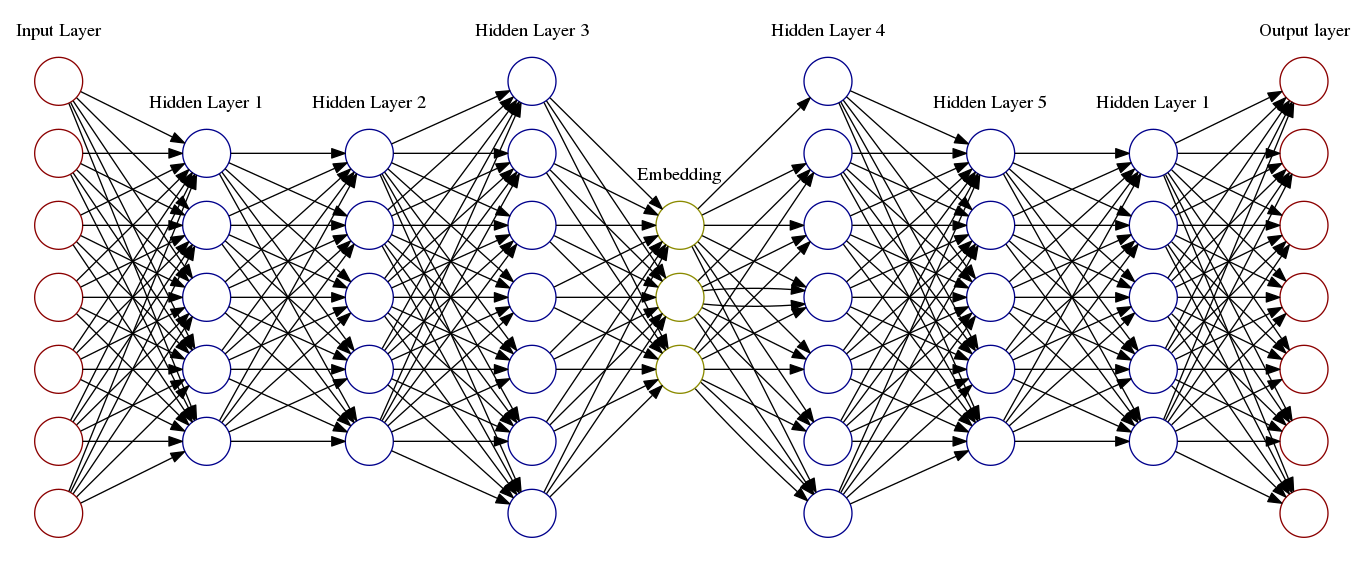
\includegraphics[scale=0.2]{archi.png}}
  \caption{\label{fig:archi}Architecture}
\end{figure}
\end{frame}

\begin{frame}
\frametitle{Hyperparameters}
\begin{table}[!h]
\centering
\resizebox{\textwidth}{!}{%
  \begin{tabular}{| l | l | l | l |}
    \hline
               & 20NEWS Without noise & 20NEWS With noise & RCV1 Without noise  \\ \hline
    $\lambda$  & $10^{-1}$            & $10^{-1}$         & $10^{-2}$           \\ \hline
    $\alpha_0$ & $10^{-2}$            & $5.10^{-3}$       & $10^{-1}$           \\ \hline
    $\alpha_1$ & 0                    & 0                 & 0                   \\ \hline
    $\alpha_2$ & 0                    & 0                 & 0                   \\ \hline
    $\eta$     & 0                    & 0                 & 0                   \\ \hline
  \end{tabular}
}
\end{table}
\end{frame}

\begin{frame}
\frametitle{Results}
\begin{table}[!h]
\resizebox{\textwidth}{!}{%
  \begin{tabular}{| l |l | l | l| l | l | l | l | l | l | }
    \hline
    & \multicolumn{3}{|c|}{20NEWS Without noise} & \multicolumn{3}{|c|}{20NEWS With noise}             & \multicolumn{3}{|c|}{RCV1 Without noise}\\
    & ACC            &ARI             & NMI            & ACC           & ARI           &NMI &ACC            & ARI           &NMI \\ \hline
Deep $K$-Means &$52.0\pm 2.3$&$34.2\pm 1.7$&$50.5\pm 1.5$&$41.5\pm 2.3$&$19.8\pm 1.5$&$28.3\pm 0.8$&$52.8\pm 3$&$24.1\pm 3.9$&$30.7\pm$\\ \hline
Constrained Deep $K$-Means&\boldmath$53.3\pm 2.1$&\boldmath$35.9\pm 1.2$&\boldmath$50.9\pm 0.8$&\boldmath$43.3\pm 2.6$&\boldmath$22.1\pm 2.4$&\boldmath$31.4\pm 1.5$ &\boldmath$63.2\pm 4.7$&\boldmath$31.4\pm 3.7$&\boldmath$37.5\pm 4.4$\\ \hline
  \end{tabular}
}
\end{table}
\end{frame}

\section{Conclusion \& Future Works}

\begin{frame}
  \frametitle{Conclusion}
  We have presented and tested in this study an approach to integrate lexical 
\end{frame}

\begin{frame}
\frametitle{Future Works}
\begin{itemize}
\item Test pairwise constraints
\item More baseline Algorithm
\item Rebustness
\end{itemize}
\end{frame}

\begin{frame}
Any Questions ?
\end{frame}

\end{document}
